\documentclass[border=5pt]{standalone}
\usepackage{tikz}
\usetikzlibrary{shapes,arrows.meta,positioning,backgrounds,fit,calc,decorations.pathreplacing,shadows}
\usepackage{amsmath,amssymb}
\usepackage{xcolor}

% Colour palette
\definecolor{inputcol}{RGB}{66,133,244}    % blue
\definecolor{memcol}{RGB}{171,71,188}       % purple
\definecolor{routecol}{RGB}{255,167,38}     % orange
\definecolor{modcol1}{RGB}{66,165,245}      % light blue
\definecolor{modcol2}{RGB}{102,187,106}     % green
\definecolor{modcol3}{RGB}{239,83,80}       % red
\definecolor{modcol4}{RGB}{255,202,40}      % yellow
\definecolor{outputcol}{RGB}{38,166,154}    % teal
\definecolor{errcol}{RGB}{229,57,53}        % error red
\definecolor{bgmodule}{RGB}{245,245,250}
\definecolor{bgroute}{RGB}{255,248,235}

\begin{document}
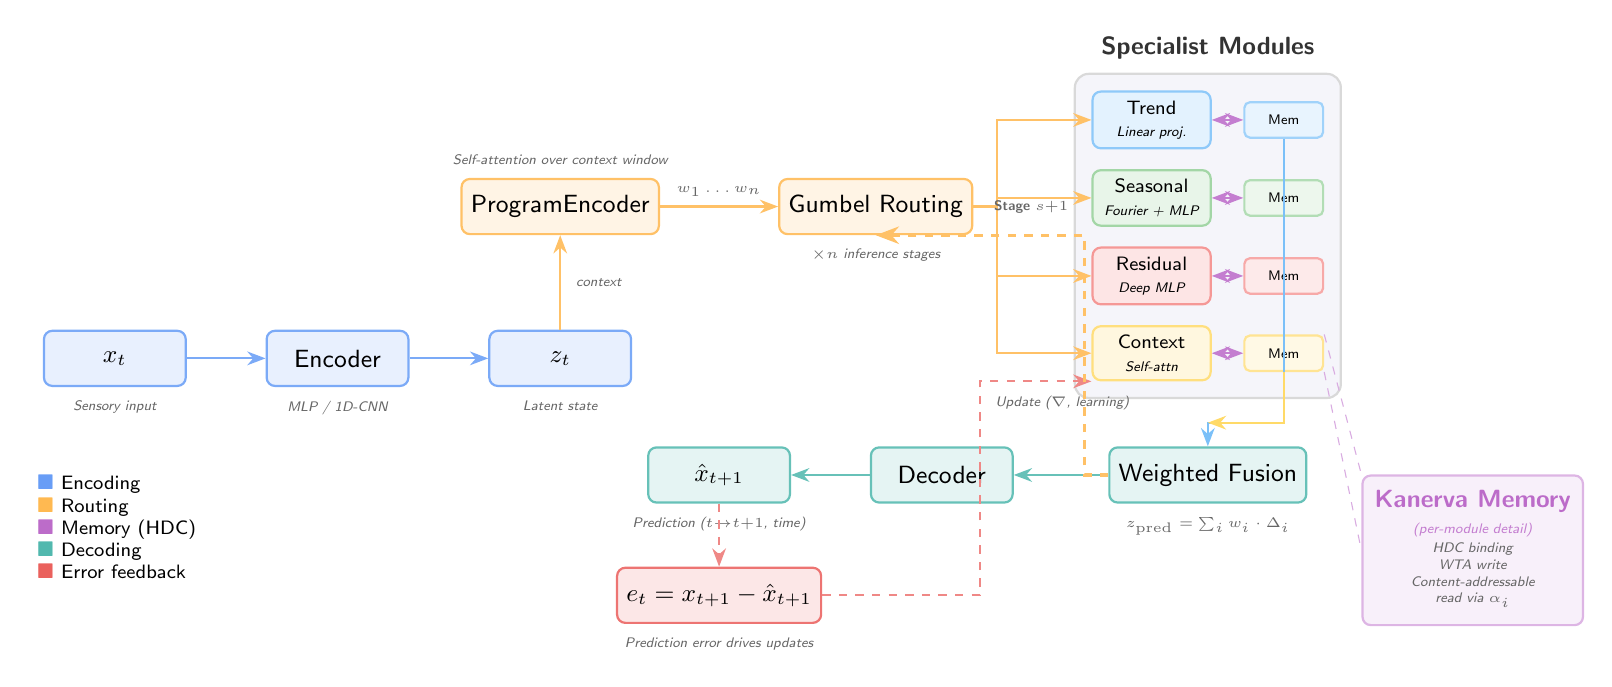
\begin{tikzpicture}[
    >=Stealth,
    node distance=0.6cm and 0.8cm,
    box/.style={draw, rounded corners=3pt, minimum height=0.7cm, minimum width=1.8cm,
                font=\small\sffamily, thick, fill=#1!12, draw=#1!70},
    box/.default=inputcol,
    membox/.style={draw, rounded corners=3pt, minimum height=0.55cm, minimum width=1.3cm,
                   font=\scriptsize\sffamily, thick, fill=memcol!15, draw=memcol!60},
    modbox/.style={draw, rounded corners=3pt, minimum height=0.6cm, minimum width=1.5cm,
                   font=\scriptsize\sffamily, thick, fill=#1!15, draw=#1!60},
    smallbox/.style={draw, rounded corners=2pt, minimum height=0.45cm, minimum width=1.0cm,
                     font=\tiny\sffamily, thick, fill=#1!12, draw=#1!50},
    arr/.style={->, thick, color=#1!70},
    arr/.default=black,
    darr/.style={->, thick, dashed, color=#1!60},
    label/.style={font=\tiny\sffamily\itshape, color=black!60},
    biglabel/.style={font=\small\sffamily\bfseries, color=black!80},
]

% ============ INPUT ============
\node[box=inputcol] (input) {$x_t$};
\node[label, below=0.05cm of input] {Sensory input};

% ============ ENCODER ============
\node[box=inputcol, right=1.0cm of input] (enc) {Encoder};
\node[label, below=0.05cm of enc] {MLP / 1D-CNN};

\draw[arr=inputcol] (input) -- (enc);

% ============ LATENT ============
\node[box=inputcol, right=1.0cm of enc] (zt) {$z_t$};
\node[label, below=0.05cm of zt] {Latent state};

\draw[arr=inputcol] (enc) -- (zt);

% ============ PROGRAM ENCODER ============
\node[box=routecol, above=1.2cm of zt] (prog) {ProgramEncoder};
\node[label, above=0.05cm of prog] {Self-attention over context window};

\draw[arr=routecol] (zt) -- node[right, label, xshift=2pt] {context} (prog);

% ============ ROUTING ============
\node[box=routecol, right=1.5cm of prog] (route) {Gumbel Routing};
\node[label, below=0.05cm of route] {$\times n$ inference stages};

\draw[arr=routecol] (prog) -- node[above, label] {$w_1 \ldots w_n$} (route);

% ============ SPECIALIST MODULES (stacked) ============
\node[modbox=modcol1, right=1.5cm of route, yshift=1.1cm, align=center] (mod1) {Trend\\{\tiny\itshape Linear proj.}};
\node[smallbox=modcol1, right=0.4cm of mod1] (mod1m) {Mem};

\node[modbox=modcol2, below=0.25cm of mod1, align=center] (mod2) {Seasonal\\{\tiny\itshape Fourier + MLP}};
\node[smallbox=modcol2, right=0.4cm of mod2] (mod2m) {Mem};

\node[modbox=modcol3, below=0.25cm of mod2, align=center] (mod3) {Residual\\{\tiny\itshape Deep MLP}};
\node[smallbox=modcol3, right=0.4cm of mod3] (mod3m) {Mem};

\node[modbox=modcol4, below=0.25cm of mod3, align=center] (mod4) {Context\\{\tiny\itshape Self-attn}};
\node[smallbox=modcol4, right=0.4cm of mod4] (mod4m) {Mem};

% Memory arrows
\draw[arr=memcol, <->] (mod1) -- (mod1m);
\draw[arr=memcol, <->] (mod2) -- (mod2m);
\draw[arr=memcol, <->] (mod3) -- (mod3m);
\draw[arr=memcol, <->] (mod4) -- (mod4m);

% Routing arrows to modules
\draw[arr=routecol] (route.east) -- ++(0.3,0) |- (mod1.west);
\draw[arr=routecol] (route.east) -- ++(0.3,0) |- (mod2.west);
\draw[arr=routecol] (route.east) -- ++(0.3,0) |- (mod3.west);
\draw[arr=routecol] (route.east) -- ++(0.3,0) |- (mod4.west);

% ============ BACKGROUND: Modules group ============
\begin{scope}[on background layer]
  \node[fit=(mod1)(mod1m)(mod4)(mod4m), fill=bgmodule, rounded corners=5pt,
        inner sep=6pt, draw=black!15, thick] (modgroup) {};
  \node[biglabel, above=0.05cm of modgroup.north] {Specialist Modules};
\end{scope}

% ============ FUSION ============
\node[box=outputcol, below=0.6cm of modgroup.south] (fuse) {Weighted Fusion};
\node[label, below=0.05cm of fuse] {$z_{\mathrm{pred}} = \sum_i w_i \cdot \Delta_i$};

% Module outputs to fusion
\coordinate (fusein) at ($(fuse.north) + (0, 0.3)$);
\draw[arr=modcol1] (mod1m.south) |- (fusein) -- (fuse.north);
\draw[arr=modcol4] (mod4m.south) |- (fusein);

% ============ DECODER ============
\node[box=outputcol, left=1.2cm of fuse] (dec) {Decoder};

\draw[arr=outputcol] (fuse) -- (dec);

% ============ OUTPUT ============
\node[box=outputcol, left=1.0cm of dec] (output) {$\hat{x}_{t+1}$};
\node[label, below=0.05cm of output] {Prediction ($t{\to}t{+}1$, time)};

\draw[arr=outputcol] (dec) -- (output);

% ============ PREDICTION ERROR ============
\node[box=errcol, below=0.8cm of output] (err) {$e_t = x_{t+1} - \hat{x}_{t+1}$};
\node[label, below=0.05cm of err] {Prediction error drives updates};

\draw[darr=errcol] (output) -- (err);

% Error feedback arrow (curved, back to modules)
\draw[darr=errcol] (err.east) -- ++(2.0,0) |- node[right, label, xshift=2pt, yshift=-8pt] {Update ($\nabla$, learning)} (mod4.south west);

% ============ HDC MEMORY DETAIL (magnifier callout from one Mem chip) ============
\node[draw, rounded corners=3pt, minimum height=1.9cm, minimum width=2.8cm,
      fill=memcol!8, draw=memcol!40, thick,
      below=1.3cm of mod4m, xshift=2.4cm] (hdcbox) {};
\node[biglabel, memcol!80] at (hdcbox.north) [anchor=north, yshift=-2pt] {Kanerva Memory};
\node[font=\tiny\sffamily\itshape, color=memcol!70] at (hdcbox.north) [anchor=north, yshift=-14pt] {(per-module detail)};
\node[label, text width=2.5cm, align=center] at (hdcbox.center) [yshift=-9pt] {
  HDC binding\\
  WTA write\\
  Content-addressable\\
  read via $\alpha_i$
};

% zoom/magnifier expansion lines: this box details ONE Mem chip
\draw[dashed, thin, memcol!45] (mod4m.north east) -- (hdcbox.north west);
\draw[dashed, thin, memcol!45] (mod4m.south east) -- (hdcbox.west);

% ============ ITERATION ARROW ============
\draw[arr=routecol, very thick, dashed] (fuse.west) -- ++(-0.3,0) |- node[left, label, xshift=-2pt, yshift=10pt] {\textbf{Stage $s{+}1$}} (route.south);

% ============ LEGEND / ANNOTATION ============
\node[font=\scriptsize\sffamily, text width=3cm, align=left, anchor=north west]
  at ($(input.south west) + (-0.2, -1.0)$) {
  \textcolor{inputcol!80}{$\blacksquare$} Encoding\\
  \textcolor{routecol!80}{$\blacksquare$} Routing\\
  \textcolor{memcol!80}{$\blacksquare$} Memory (HDC)\\
  \textcolor{outputcol!80}{$\blacksquare$} Decoding\\
  \textcolor{errcol!80}{$\blacksquare$} Error feedback
};

\end{tikzpicture}
\end{document}
